\documentclass[a4paper,twoside,openleft,12pt]{filipecorreiathesis} % define the title 
\usepackage[a4paper,margin=2.5cm, top=3cm, bottom=3cm]{geometry} % use bindingoffset=2cm for binding
\usepackage{appendix}
\usepackage{makeidx}
\usepackage{fancyhdr}
\usepackage{amsfonts, amssymb, amsthm, mathrsfs}
\usepackage{multicol}
\usepackage{multirow}
\usepackage{setspace} 
\usepackage{xspace}
\usepackage{algorithm, algorithmicx, algpseudocode}
\usepackage{rotating}
\usepackage{courier}
\usepackage{textcomp}
\usepackage{booktabs}
\usepackage{bookmark}
\usepackage[ISBN=555-555-555-555-0,SC0]{ean13isbn}
\usepackage{wrapfig}
\usepackage{soul} % provides yellow-marker highlighting among other features
\usepackage{verbatim} % provides the 'comment' environment among other features
\usepackage{xifthen} % provides \ifthenelse 

\usepackage{enumitem}
\usepackage{pbox}
\usepackage[section]{placeins} % stops floats (figures, tables...) to appear outside the section where they are placed.
\usepackage{cleveref}[2012/02/15]

\usepackage{longtable}
\usepackage{subcaption}

\usepackage{calligra}
\newcommand{\setfont}[2]{{\fontfamily{#1}\selectfont #2}}


\makeindex

% dividing diamonds
\newcommand{\dividingdiamonds}{\vspace{0.2cm}\centerline{$\diamond \diamond \diamond$}\vspace{0.2cm}}%


%\onehalfspacing
\setstretch{1.3} % for custom spacing

% indentation of multiline figure/table captions.
%\usepackage[format=plain,justification=RaggedRight]{caption}

% Vertically centered table columns
\newcolumntype{M}{>{\centering\arraybackslash}m{\dimexpr.25\linewidth-2\tabcolsep}}

%% Fixes problem with bibliograpy key protruding into description
\usepackage{eqparbox}
\usepackage[numbers]{natbib}
\renewcommand*{\bibnumfmt}[1]{\eqparbox[t]{bblnm}{[\textcolor{feup}{#1}]}}

\def\isnum#1{%
  \if!\ifnum9<1#1!\else_\fi
    \oldstylenums{#1}\else#1\fi}

%% Fancy Headers -- Somehow, I can't seem to be able to move this to the .cls file
\pagestyle{fancy}
\fancyhf{}
\fancyhead[LE]{\small \leavevmode\llap{\textcolor{feup}{\isnum{\thepage}}\hspace{0.5cm}}\smallcaps{\leftmark}}
\fancyhead[RO]{\small \leavevmode\smallcaps{\rightmark}\rlap{\hspace{0.5cm}\textcolor{feup}{\isnum{\thepage}}}}
\fancypagestyle{plain} {
 \fancyhf{} % get rid of headers on plain pages
 \renewcommand{\headrulewidth}{0pt} % and the line
 \renewcommand{\footrulewidth}{0pt} % and the line
}
\renewcommand{\headrulewidth}{0pt}
\renewcommand{\footrulewidth}{0pt}
\setlength\headsep{1.1cm}
\setlength\headheight{13.6pt}

\renewcommand{\chaptermark}[1]{\markboth{#1}{}}
\renewcommand{\sectionmark}[1]{\markright{#1}{}}

%% Define a new 'leo' style for the package that will use a smaller font.
\usepackage{url}
\makeatletter
\def\url@leostyle{%
  \@ifundefined{selectfont}{\def\UrlFont{\sf}}{\def\UrlFont{\footnotesize\ttfamily}}}
\makeatother
\urlstyle{leo}

%\usepackage{inconsolata} % monospace font, used for \texttt{}


\begin{document}
	\title{Thesis title}
	\author{\href{mailto:your-email-address@fe.up.pt}{Your Full Name}}

	\frontmatter
	    \pagestyle{empty}
	    \maketitle
		\noindent\textbf{Contact Information:} \\

\noindent Pedro Miguel Lourenço Costa \\
Faculdade de Engenharia da Universidade do Porto \\
Departamento de Engenharia Informática \\

\noindent Rua Dr. Roberto Frias, s/n \\
4200-465 Porto \\
Portugal \\

\noindent Tel.: +351 968 203 386 \\
Email: pedro.miguel.costa@fe.up.pt \\
URL: https://www.linkedin.com/in/pedro-costa-3279996b \\

\vfill


		\cleardoublepage
		\begin{flushright} 
  %\null\vspace{\stretch{1}}
  \null
  \vfill
  \emph{\Large{\dots to the world in general}} \\
  \vspace{3cm}
\end{flushright}
		\clearpage
		{\centering \emph{This page was intentionally left blank.} \\ }
		\dominitoc
		\cleardoublepage
		\pagenumbering{roman}
		\pagestyle{fancy}
		\chapter{Abstract}


Nowadays, nearly every medium-size or large company in the electronics, pharmaceutics, food, or other industries needs to support its operations by managing the exchanged information and resources. The upstream and downstream flow of these, together with the system of organizations, people and activities that make it possible, is commonly referred to as a supply chain. In a practical sense, a supply chain’s flow of products and services goes from supplier to consumer. For example, the supermarket fish a person eats: it is caught in boats, then prepared, and distributed to a store where the final consumer is able to buy it. But supply chains are becoming very complicated and complex systems, spanning multiple businesses and relationships, interlaced in many different ways, which is a reason why supply chain management (SCM), the discipline which deals with the coordination of a supply chain, is becoming increasingly more important.  The information has to flow through the chain, sometimes even reverting the direction, but the paths it takes are not always very obvious or even traceable in the global context, dealing with many issues along the way.

Managing inventory and suppliers while maintaining safety, quality and keeping to the schedule is a difficult task. Delays are common, and a company’s finances, growth and reputation are affected. This is further aggravated by the fact that information is not always accurate or available when needed. And the fact that companies value their privacy makes it so that sharing information with others is not always simple or desirable. 

Most important of all, frequently, there are big holes of information in a supply chain, analog gaps where the information has not been made digital in the system. The use of traditional tools is still too prevalent. Emails are sent, documents are printed and mailed, instead of making the information digital, putting  it directly on the network and relaying it to the next link in the chain. This fact, together with the sometimes apparent lack of interoperability between the SCM software of different companies and their need to protect their private information is what makes a global overview of the whole chain complicated with the current technologies. Provenance and traceability of a supply chain are a big objective for companies, along with improving security, efficiency and effectiveness of the supply chains.

Most of these issues are, in great part, caused by the standalone use of outdated or inadequate software architectures, which, traditionally, are often centralized and have single points of failure. And even when they are not, oftentimes they are insecure, prone to synchronization problems, leading to big delays in both relaying the information and resources and making payments possible. 

One way to approach these specific problems of supply chains that are brought by the traditional IT solutions is to update them with new infrastructures, namely by using blockchain technology. Blockchain is a decentralized technology that has no single point of failure and allows for the immutable storage of verifiable data all over the computers that store it. Each time there is a new piece of information, its validity is verified by the network and it is inserted into a block of the chain, which leads it to being continually extended. This means that we can check all the information that there ever was, since the beginning, and validate it easily, or make any necessary calculations. As such, blockchains are the perfect means to achieve traceability of a supply chain. At the same time they are a secure and incorruptible way to store information, with a fast synchronization time, being perpetually available to anyone, anywhere within the network. It would also be the way to close the analog gaps, turning the chain fully digital, leading to the possibility of a global overview.

This project focuses on researching the effects of applying blockchain technology to a supply chain and its management. By doing this, it should be possible to ascertain how much this technology can really impact SCM over the traditional IT solutions, or in combination with them. A practical instance involving the application of this technology to a system will also be developed, to further demonstrate its possible benefits.

The improvements that it could bring are, however, not limited to the problems described. Blockchain is a whole new game, and it brings a whole new myriad of possibilities into the table. We are only seeing the tip of the iceberg and this is an area that is of the interest of any company which aims to improve the efficiency and effectiveness of its entire supply chain system.

\textbf{Keywords:} Supply Chain, Supply Chain Management, Industry, Blockchain, Network, Decentralization, Security, Traceability, Provenance, Information Integration, Ledger, Interoperability


\chapter{Resumo}

Tradução PT do abstract





		\addtocontents{toc}{\protect{\pdfbookmark[0]{\contentsname}{toc}}}
		\tableofcontents
		\cleardoublepage
		\phantomsection
		\addcontentsline{toc}{chapter}{\listfigurename}
		\listoffigures
		\cleardoublepage
		\phantomsection
		\addcontentsline{toc}{chapter}{\listtablename}
		\listoftables
		\cleardoublepage
		\chapter{Preface}

\epigraph{\emph{
A quote
}}{\sc The Quote's Author}
\vspace{1pc}


Lorem ipsum



	\mainmatter

	% final lineup
	%\chapter{Introduction1}
%\minitoc \mtcskip \noindent
%\chapter{Introduction2}
%\minitoc \mtcskip \noindent
\chapter{Introduction}
\label{chap:introduction}
\minitoc \mtcskip \noindent

Our society is turning more consumerist, with most people in developed countries having high consumer power and standards of life. Consumers goods, from the essentials up until the entertainment goods, are manufactured and ordered continuously in high quantities.

Modern supply chains feel the pressure of this growth, leading to the demand for an efficient management. Most companies are making efforts towards this end, and, even though part of the answer to an efficient management lies in having efficient processes, a good management is also based in using the right technologies. Thus, the development of technologies that can satisfy the demands of supply chain management, for any industry, is in high demand.

%The development of such technologies should be faced towards the problems that supply chains 

%ace concerns are raised as to whether the demand can be met in a transparent and trustful way. It is difficult to know where the products we consume come from, and the processes they go through. This leads to the need of transparency in the supply chains as well as the need of an increase in their efficiency, if they are to conform to the market's needs.

\section{Supply Chains}
\label{supply_chains}
\textbf{Supply Chains} can be found, in some form, in nearly every business, spanning many different areas of operation. Traditionally, a supply chain encompasses all the processes and activities that lead from the initial raw materials to the final finished product, as well as all the functions and services within and outside a company. A supply chain can also be defined as the network of entities through which material flows. These entities can be identified as suppliers, carriers, manufacturing sites, distribution centers, retailers, and customers~\cite{Lummus2014}. Naturally, with the upstream and downstream flow of these materials and resources, comes a lot of information on them and on the processes, people and organizations they are associated with. Realistically, the  flow is not always arborescent, as there are many considerations to be taken and decisions to be made. Supply chains have multiple end products with shared components, facilities and capacities~\cite{Ganeshan1995}. As a consequence, the paths taken by the resources and information are not straightforward, but interlace, diverge and converge at different points, go back and forth, as exemplified in Figure~\ref{fig:supplychain_complexity}.
  
\begin{figure}[ht]
\centering
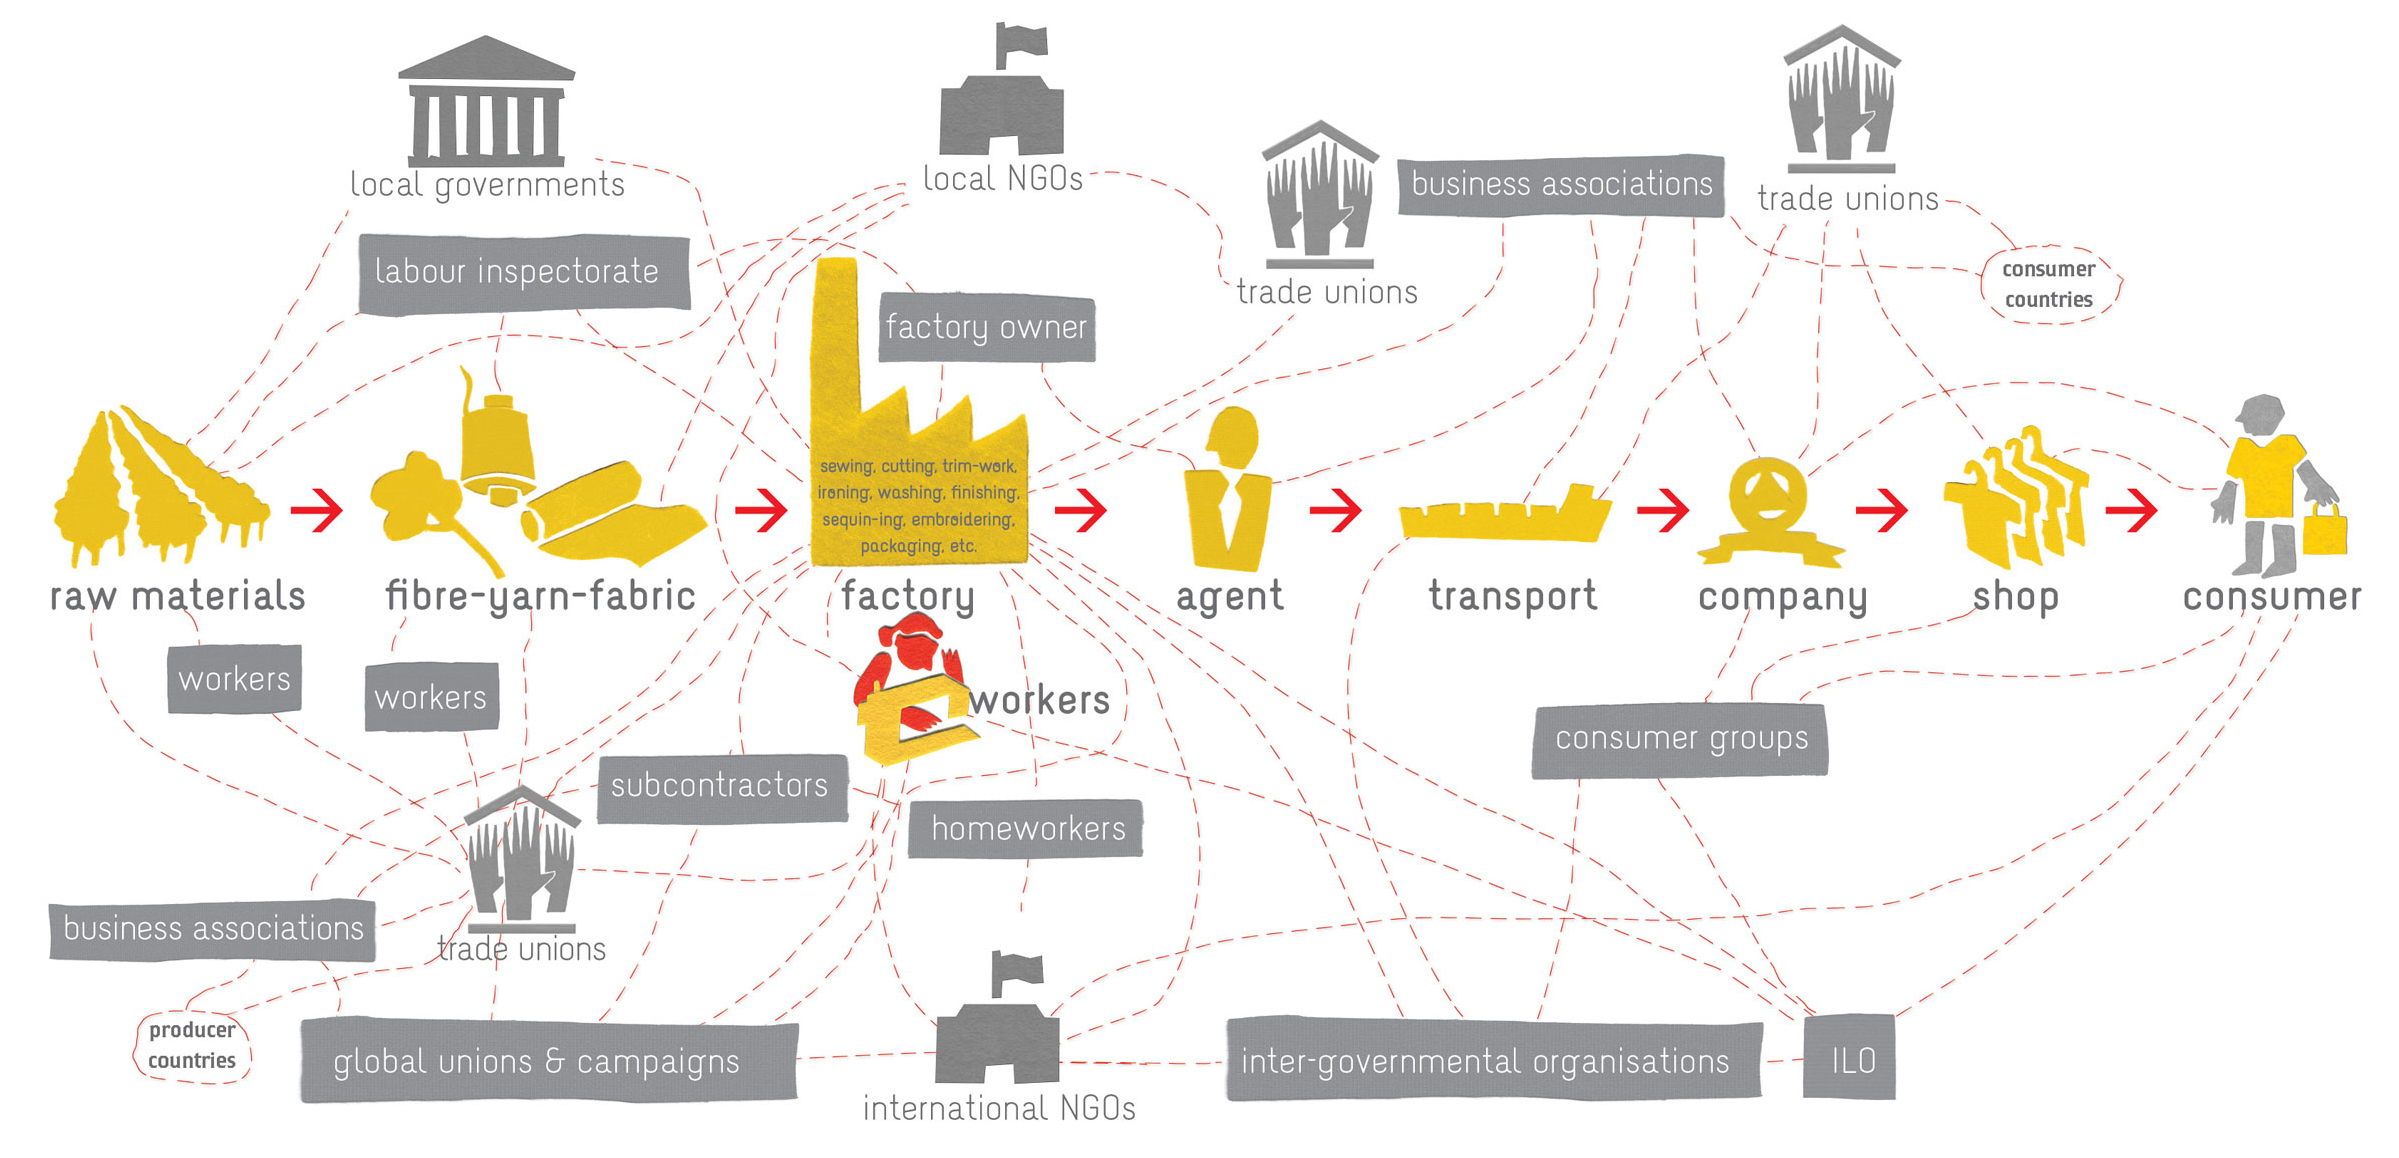
\includegraphics[scale=0.18]{media/supplychain_complexity.jpg}
\caption[Representation of a garment supply chain and all the relationships it involves]{Representation of a garment supply chain and all the relationships it involves. Taken from the International Training Centre of the International Labour Organization briefing on global supply chains~\cite{ITCILO2018}.}
\label{fig:supplychain_complexity}
\end{figure}
  
  The activities and processes a supply chain encompasses include: sourcing raw materials and parts, manufacturing and assembly, warehousing and inventory tracking, order entry and order management, distribution across all channels, delivery to the customer, and managing the information systems necessary to monitor all of these activities. As Lummus~\cite{Lummus2014} describes, these activities can be roughly mapped to the 4 essential processes: plan, source, make, deliver.
    
  Coordinating all of these is no easy task, and so the discipline of SCM comes into life. According to Ballou~\cite{Ballou2007}, the Council of SCM Professionals (CSCMP) defines SCM as \textit{“the planning and management of all activities involved in sourcing and procurement, conversion, and all Logistics Management activities. Importantly, it also includes coordination and collaboration with channel partners, which can be suppliers, intermediaries, third-party service providers, and customers. In essence, SCM integrates supply and demand management within and across companies”}.

From this definition follows that SCM deals a lot with both coordination and collaboration between entities, and so, the management of the flow of information and resources between them is very important. The objective is always, of course, to minimize the total cost of these flows between and among stages~\cite{Habib2011}.
In the end, the creation of value (products and services) in a supply chain stems from the relationships that different entities build between themselves, and not from the work of a single entity. As such, supply chains, not firms, compete and those which have the best integration and management processes win.

And this is where SCM shines and shows just how useful it can be. Managing all the processes in a supply chain, while maintaining safety, quality and keeping to schedule is difficult. An event on one side of the world, large or small, be it from human or natural causes, can easily disrupt the links in the supply chain. For instance, it might disrupt the supply of a critical component or service. Delays are, therefore, common, and the consequences of such disruptions might have a severe impact in the finances, growth and reputation of the companies involved~\cite{Punter2013}.

SCM diminishes the impact of such disruptions, and actively works to avoid or diminish them, while optimizing the way the supply chain works. This is why SCM is such an important discipline, that we have to better understand and improve, with all the means that we can, and this includes, of course, research into technologies like the blockchain.

\section{Challenges}
\label{sec:supply-chain-challenges}

 Having already introduced the concepts of Supply Chain and SCM, it is now possible to briefly introduce some of the problems that affect them.

The first, and most generalist problem of a supply chain, is the ease with which \textbf{an unexpected event might cause delays}. These events, already mentioned in Section~\ref{supply_chains} are not always predictable and must be contained as fast as possible. One event in particular which, often, causes delays are \textbf{synchronization problems in the processes and information systems of a company}~\cite{Prokle2017}. 

    Another problem is that, often, there are difficulties in sharing information between companies. This is caused both by the fact that \textbf{companies value their privacy and the security of their information}, which means they might not want to share too much information, or that they might only share it through secure channels, and by the \textbf{lack of standards for sending information and communicating}~\cite{Korpela2017}. The issue with non-existing standards is that companies are left to discuss what details to share or not, wasting time and resources.

Most important of all, in the industry, \textbf{the use of traditional tools and manual work is still too prevalent}. Emails are sent, documents are printed and mailed, instead of transmitting the information in a more automatic, direct and secure way through the network. This point also brings the next problem of supply chains to light: the apparent lack of interoperability between certain softwares (which might be a byproduct of by the lack of standards).
 
 
Finally, provenance and traceability of the products on a supply chain are a big objective for companies. But \textbf{the current technologies used in supply chain only accomplish provenance and traceability in a limited scope}, as the information a certain entity possesses is usually also limited. And so, it is very hard for anyone to have a global overview of the supply chain.

Though it is not proven, it is be possible that some, if not most, of these issues in supply chain might be caused by the use of software architectures that do not allow for full data integration. An optimal supply chain should be as efficient and effective as possible, while being secure and satisfying all the traceability requirements. Perhaps, it is time to try out new solutions which replace or augment the existing ones, in such a way that supply chain management can better satisfy the needed requirements.

\section{From Blockchain Technologies to Supply Chains} \label{sec:context}

Blockchain technology allows for secure, public, distributed and decentralized systems. Though it was first proposed in its actual form by Satoshi Nakamoto~\cite{Nakamoto2008}, an anonymous group which published a white paper in 2008, this was not the first reference to such a technology. The first work on a cryptographically secured chain of blocks was described in 1991 by Stuart Haber and W. Scott Stornetta~\cite{Haber1991}, and further refined in 1992 by Bayer \& Haber, by incorporating Merkle trees~\cite{Bayer1993}. Since then, it has come a long way, sprouting multiple different uses and applications of the technology. Its characteristics make the development of distributed and permanently, globally available systems possible, which is a paradigm that is attracting the interest of various industries.

One area in particular where we believe blockchain could bring about great improvements is Supply Chain Management (SCM). SCM has seen an increase in complexity in the last few decades, due to the globalization of the market, with businesses interlacing in many different ways, their relations extending way beyond what they used to, as found by Filiz Isik~\cite{Isik2011}. This increase in complexity is somewhat hard to manage and some supply chains stretch and encompass so many businesses that, due to their software not being prepared for this, the information is not always transmitted from end to end, leaving holes of information in between the links that join each business, thus leading to a lot of chaos and uncertainty as to the state of the key items in the chain~\cite{Wilding1998}.

   This dissertation work will focus on supply chain management, and on how blockchains can possibly be applied to improve this area, leading to positive impacts in the logistics industry and eventually finding benefits for the consumer as well. 

%%%%%%%%%%%%%%%%%%%%%%%%%%%%%%%%%%%%%%%%%%%%%%%%%%%%%%%%%%%%%%%%%%%

\section{Motivation} 
\label{sec:motivation}

As described in section~\ref{sec:supply-chain-challenges}, a possible cause of these problems might be the use of software that can not keep up with the evolution of the requirements of modern supply chains. Today's supply chains have high standards for their requirements and even when the software works just fine, maybe it is not recent enough or it was not specified and built to satisfy these requirements. For instance, product falsification might be a huge issue nowadays in the supply chain, but maybe it was not rated as a high importance problem 15 years ago. Therefore, the software from 15 years ago complied with different requirements than the ones from today and was not built to handle that specific problem well. 

\textbf{Requirements evolve, and so should the technology, in order to support them.} There is an immediate need for solutions, which might either completely replace the previous ones, or augment them.

One way to approach these specific problems is to research what would a modern requirements specification for supply chain look like, and develop new technologies that are more accurately specified for the supply problem challenges in question. 

The characteristics of blockchain architectures seem to be a good solution for many of the identified problems in supply chain to be reduced or neutralized. These architectures are the perfect means to achieve traceability of a supply chain, and so, they are good to achieve provenance as well. At the same time they are a secure, incorruptible and immutable way to store information, with a fast synchronization time, being perpetually available to anyone who has permission, anywhere within the network. It would also be the way to close the analog gaps, turning the chain fully digital, leading to the possibility of a global overview.

\section{Objectives}
\label{sec:objectives}
The main objective of this dissertation is to find whether blockchain technology is a good fit to solve the most common problems of supply chain management, and also to find out the technological requirements of a modern supply chain. There are a multitude of small tasks that blockchain could automatize in supply chain, so this thesis will try to figure out which ones blockchain applies to better. 

The primary objective of this dissertation is determining if blockchain architectures can be successfully applied to supply chain management as an improvement towards the technologies that are already being used. For this purpose, it is necessary to conduct research on the supply chain issues and validate these, in order to propose a blockchain design that can target these issues successfully. 

\section{Dissertation Structure} \label{sec:struct}

Besides the introduction, this dissertation has 6 more chapters, divided into 2 parts.

\par \textbf{Part 1: Background and State of the Art} - Provides the needed concepts to understanding the work, as well as explanations about the existing tools and projects related to the blockchain and to its application to supply chain management domain.
 The state of the art is divided into 2 chapters:~\ref{chap:blockchain} and ~\ref{chap:blockchain-applicability}.
\begin{itemize}
  \item Chapter~\ref{chap:blockchain}, "Blockchain Technologies", some important concepts from the blockchain architecture are presented and discussed, followed by an analysis of the existing blockchain networks and frameworks and their comparison.
  \item Chapter~\ref{chap:blockchain-applicability}, "Blockchain in the Industry", the application of blockchain to supply chain is discussed in more detail, including the possible advantages, challenges, and following it up with an analysis of the existing blockchain applications that also focus on supply chain. 
\end{itemize}

\par \textbf{Part 2: Problem, Research and Solution} - Provides a thorough explanation of the problem, objectives and the proposed methodology to approach them. Follows up with a survey and requirements analysis, which serves as a base to propose a blockchain solution design. 
\begin{itemize}
  \item Chapter~\ref{chap:supply-chain-problems}, "Problem Statement", specifies the thesis statement and the questions that need to be answered in order to reach a conclusion.
  \item Chapter~\ref{chap:survey}, "Supply Chain Issues Validation and Requirements Elicitation", features a survey and the analysis of its results, such as to gather the requirements for a supply chain system, so that a blockchain-based solution can be proposed.
  \item Chapter~\ref{chap:prototype}, "Solution Design and Implementation", features the choice of a blockchain framework and the proposal of a solution, which consists in building a proof of concept (PoC) project that implements the requirements elicited from the survey.
\end{itemize}

\par \textbf{Part 3: Conclusion} - Gathers all the information from the results of the solution to make a statement, also listing contributions, difficulties and future work.
\begin{itemize}
  \item Chapter~\ref{chap:conclusions}, "Conclusions", features an overview of the work done in the dissertation, providing an answer to the previously defined problem, and following it up with possibilities of future work in this area.
\end{itemize}
	%\include{state-of-the-art-review}
	%\chapter{Applied designs for a blockchain driven supply chain}
\label{chap:problem}
% RESEARCH PROBLEMS

%\minitoc \mtcskip \noindent

Here, we talk concretely of the problem we will be researching. What will we be trying to figure out, to later implement? In this case, it is the designs for the blockchain

\section{Applied to the ledger}

\section{Applied to smart contracts}
	%\include{contribution1}
	%\include{contribution2}
	%\include{validation}
	\chapter{Conclusions}
\label{chap:conclusions}

\minitoc \mtcskip \noindent

%These conclusions are for PDIS; so they will close this delivery and may anticipate the expected results of the dissertation. Include the tasks and a Gantt diagram with the plan.
The dissertation focuses on finding out how applicable blockchain is to the supply chain industry and to SCM, and there are many variables to consider. Many companies have already started working on projects similar to what is trying to be accomplished here, though with a higher focus on financial benefits than on the research itself (many of the examples given were of companies using Ethereum and its tokens). These solutions have not yet been proved and are also taking their initial steps. The main focus of this dissertation is to develop a proof-of-concept that indeed blockchain can improve SCM in some form, and also give an insight on how this might be achieved. 

\section{Future Work}

The research for this dissertation is divided into six steps, described in Table \ref{table:gantt_chart} and illustrated by Figure \ref{fig:gantt_chart}. The research started with the literature review, which presents some important insights, frameworks as well as some important design aspects and decisions to take while developing a model for a blockchain-driven supply chain project.

These aspects will be taken into account for the next steps. First, adapting and creating a blockchain integration model, by making some decisions on the design and frameworks to be used. Then, a small integration project will be built based on this model.

In the final part of the project, its applicability and performance will be evaluated. The developed system itself is a proof-of-concept, which, already proves that such a concept might work, but it is important to measure how it fares against the traditional systems used in supply chain. This evaluation is done in two different parts: the first consists on evaluating functionality, and checking which functionalities are added or subtracted by using blockchain; the second part consists in using performance metrics to evaluate this dissertation's solution against the baseline of a traditional solution, like a centralized system. The metrics used to evaluate this include, but are not limited to:
\begin{itemize}
\item Throughput - processed transactions per second
\item Latency - average time to process a single transaction
\item Latency volatility - measure of the variety of latency
\item Security - qualitative evaluation that includes items such as immutability, denial of service resilience, trust and fraud protection, confidentiality and access control
\item Hardware requirements - how much hardware is needed, and how powerful
\item Scalability - number of nodes, transactions, users and how much the system can stretch these numbers
\end{itemize}

%\todo{fcorreia: do you have already any additional ideas about the baseline that you will be comparing to? it'd be great if you could provide a bit more detail about this; will it be a non-blockchain-based distributed system? (e.g., a microservice-based system, or a system based on a replicated datastore) Will it be simply a "normal" centralized system? Depending on the baseline that you choose the conclusions that you will be able to reach will be quite different}

Finally, the model might have to be recalibrated, taking into account the results gathered from these metrics. The values of the model might have to be changed iteratively, until a satisfying solution is achieved, if possible.

%%%%%%%%%%%%%%%%%%%%%%%% TABLE %%%%%%%%%%%%%%%%%%%%%%%%%%%%%%%%%

% Please add the following required packages to your document preamble:
% \usepackage[table,xcdraw]{xcolor}
% If you use beamer only pass "xcolor=table" option, i.e. \documentclass[xcolor=table]{beamer}
\begin{table}[]
\centering
\begin{tabular}{l|r|r|}
\cline{2-3}
                                                                                                  & \multicolumn{1}{l|}{{\color[HTML]{343434} \textbf{Starting}}} & \multicolumn{1}{l|}{{\color[HTML]{343434} \textbf{Ending}}} \\ \hline
\multicolumn{1}{|l|}{{\color[HTML]{343434} 1. Literature Review}}                                 & 1 Jan 2018                                                    & 9 Feb 2018                                                  \\ \hline
\multicolumn{1}{|l|}{{\color[HTML]{343434} 2. Decide on the features and design the model}}       & 10 Feb 2018                                                   & 5 Mar 2018                                                  \\ \hline
\multicolumn{1}{|l|}{{\color[HTML]{343434} 3. Create a small integration project}}                & 6 Mar 2018                                                    & 15 Apr 2018                                                 \\ \hline
\multicolumn{1}{|l|}{{\color[HTML]{343434} 4. Evaluate its applicability and performance}}        & 16 Apr 2018                                                   & 29 Apr 2018                                                 \\ \hline
\multicolumn{1}{|l|}{{\color[HTML]{343434} 5. Recalibrate the model's values, given the results}} & 30 Apr 2018                                                   & 14 May 2018                                                 \\ \hline
\multicolumn{1}{|l|}{{\color[HTML]{343434} 6. Finalize the dissertation document}}                & 15 May 2018                                                   & 22 Jun 2018                                                 \\ \hline
\end{tabular}
\caption{Work plan description for figure \ref{fig:gantt_chart}}
\label{table:gantt_chart}
\end{table}



%%%%%%%%%%%%%%%%%%%%%%%%%%%%%%%%%%%%%%%%%%%%%%%%%%%%%%%%%%%%%%%%
\begin{figure}[ht]
\centering
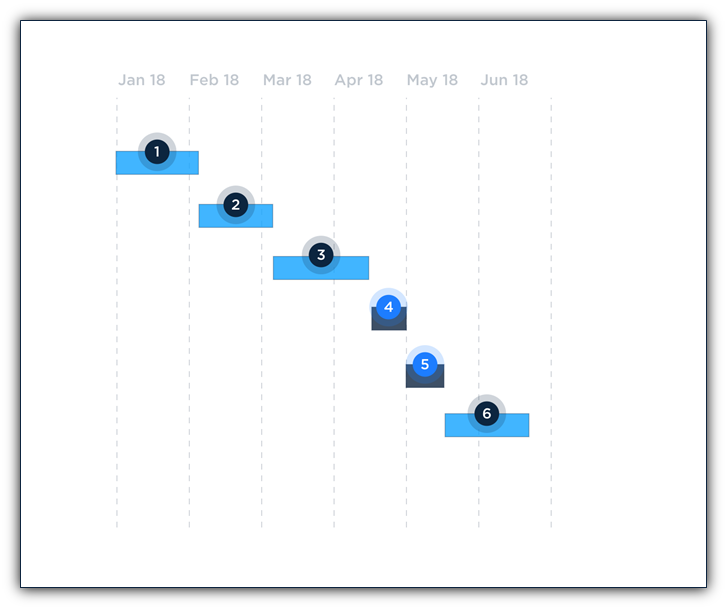
\includegraphics[scale=0.75]{media/gantt.png}
\caption{Research work plan}
\label{fig:gantt_chart}
\end{figure}

\section{Expected Results}
From this dissertation, it is expected that a proof-of-concept system with certain characteristics will emerge. The results will be analyzed to check if the system follows the parameters we are looking for.

For instance, it should be able to integrate information from various sources into a single place. This information should be available at any time, anywhere. It should be cryptographically secure, immutable, and easy and quick to share.

In the end, we need to analyze the results with the given metrics and ascertain whether there is a significant increase in performance and functionality that would justify using blockchain in a real supply chain.

%\todo{fcorreia: I'd expect to see here a list of contributions of your thesis. You do mention them, but a) I think they would be clearer to read as a list, b) you may be currently missing a few. I see at least 3 or 4, for example: a study of important design considerations for SCMSs, a study of important design considerations for blockchains, a prototype, an analysis of the benefits and liabilities of supporting a SCMS with a blockchain}

% pedro: I don't think a list is a good representation for the conclusion, especially when it is the ending of the document. And I don't know what other results to expect, I've written the ones we had discussed previously.




	\chapter*{Epilogue}
\addcontentsline{toc}{chapter}{Epilogue}  

Lorem ipsum


    \bookmarksetup{startatroot}
	\phantomsection
	\addcontentsline{toc}{part}{\appendixtocname}
	\appendixpage
	\appendix
		\chapter{Statistical Analysis Methodology}
\label{chap:appendix-a}


    % Please add the following required packages to your document preamble:
% \usepackage{multirow}
% \usepackage[normalem]{ulem}
% \useunder{\uline}{\ul}{}
\begin{table}[]
    \centering
    \caption{Data analysis metrics used in the survey results analysis}
    \label{annex:metrics}
    \resizebox{\textwidth}{!}{
    \begin{tabular}{l|l|l|}
    \cline{2-3}
                                                                                                                                 & Metrics                                                                & Meaning                                                                                                                                                                                                                                                                                                                                                                                                                                                                                                                                                                                                                     \\ \hline
    \multicolumn{1}{|l|}{\multirow{3}{*}{\begin{tabular}[c]{@{}l@{}}Measures of\\ Central Tendency \\ or Location\end{tabular}}} & \textbf{Mean}                                                          & \begin{tabular}[c]{@{}l@{}}The mean represents the most probable value. In this\\ survey, with the use of scales with a lower and upper\\ bounds, the mean has the roles of representing the\\ average value of agreement, importance and other\\ measures.Normally, when the skewness of a distribution\\ is high, the meaning of the mean may get distorted by\\ the existence of outlier values. However, since the scales\\ have a low range, with a lower and upper bound on the\\ answer values, this is not much of a concern. Therefore,\\ even in cases of skewness, the mean can be a useful metric.\end{tabular} \\ \cline{2-3} 
    \multicolumn{1}{|l|}{}                                                                                                       & \textbf{Median}                                                        & \begin{tabular}[c]{@{}l@{}}Value of the 50\% percentile, for numerical answers. Half\\ the answers are above this value and half are below,\\ pointing to a central tendency around this value. This is\\ a good metric to use, especially in skewed distributions\\ where there are outliers in the collected values, since the\\ meaning of the mean may get slightly distorted by the\\ outlier values.\end{tabular}                                                                                                                                                                                                     \\ \cline{2-3} 
    \multicolumn{1}{|l|}{}                                                                                                       & \textbf{Mode}                                                          & \begin{tabular}[c]{@{}l@{}}Most frequent response. Though it represents the most\\ popular answers, by itself the metric means nothing else,\\ as there might be answers almost as popular or not.\end{tabular}                                                                                                                                                                                                                                                                                                                                                                                                             \\ \hline
    \multicolumn{1}{|l|}{\multirow{2}{*}{\begin{tabular}[c]{@{}l@{}}Measures of Spread,\\ Scale or Dispersion\end{tabular}}}     & \textbf{\begin{tabular}[c]{@{}l@{}}Standard \\ Deviation\end{tabular}} & \begin{tabular}[c]{@{}l@{}}Quantifies the variation within the data set, by showing\\ how much the distribution spreads to either sides of the\\ center. A high value for the standard deviation means\\ that there are a lot of values away from the mean, from\\ which can be concluded that there is not a general\\ consensus on a certain answers.A low value means that\\ there is consensus, since all the values of the data set are\\ bundled more closely together.\end{tabular}                                                                                                                                  \\ \cline{2-3} 
    \multicolumn{1}{|l|}{}                                                                                                       & \textbf{Range}                                                         & \begin{tabular}[c]{@{}l@{}}Difference between highest and lowest value of the data set.\\ Together with the standard deviation, indicates the dispersion\\ of the value of the answers. A range of 0 means that a\\ question had the same value for all responses, for instance.\\ This metric ignores the frequency with which each answer\\ was given, that is why it must be coupled with the standard\\ deviation to be relevant.\end{tabular}                                                                                                                                                                          \\ \hline
    \multicolumn{1}{|l|}{\begin{tabular}[c]{@{}l@{}}Measures of\\ Skewness and\\ Kurtosis\end{tabular}}                          & \textbf{Skew}                                                          & \begin{tabular}[c]{@{}l@{}}This metric indicates the lack of symmetry in a distribution,\\ where the results bunch up in one side of the distribution.\\ For instance, negative skewness values indicate a skew to\\ the left: the values bunch up at the right end of the distribution\\ and the left tail is long, indicating there are outliers in the lower\\ values.\end{tabular}                                                                                                                                                                                                                                      \\ \hline
    \end{tabular}
    }
    \end{table}
		%\chapter{Composer Model Class Diagram}
\label{chap:appendix-b}

\begin{figure}[h]
    \centering
    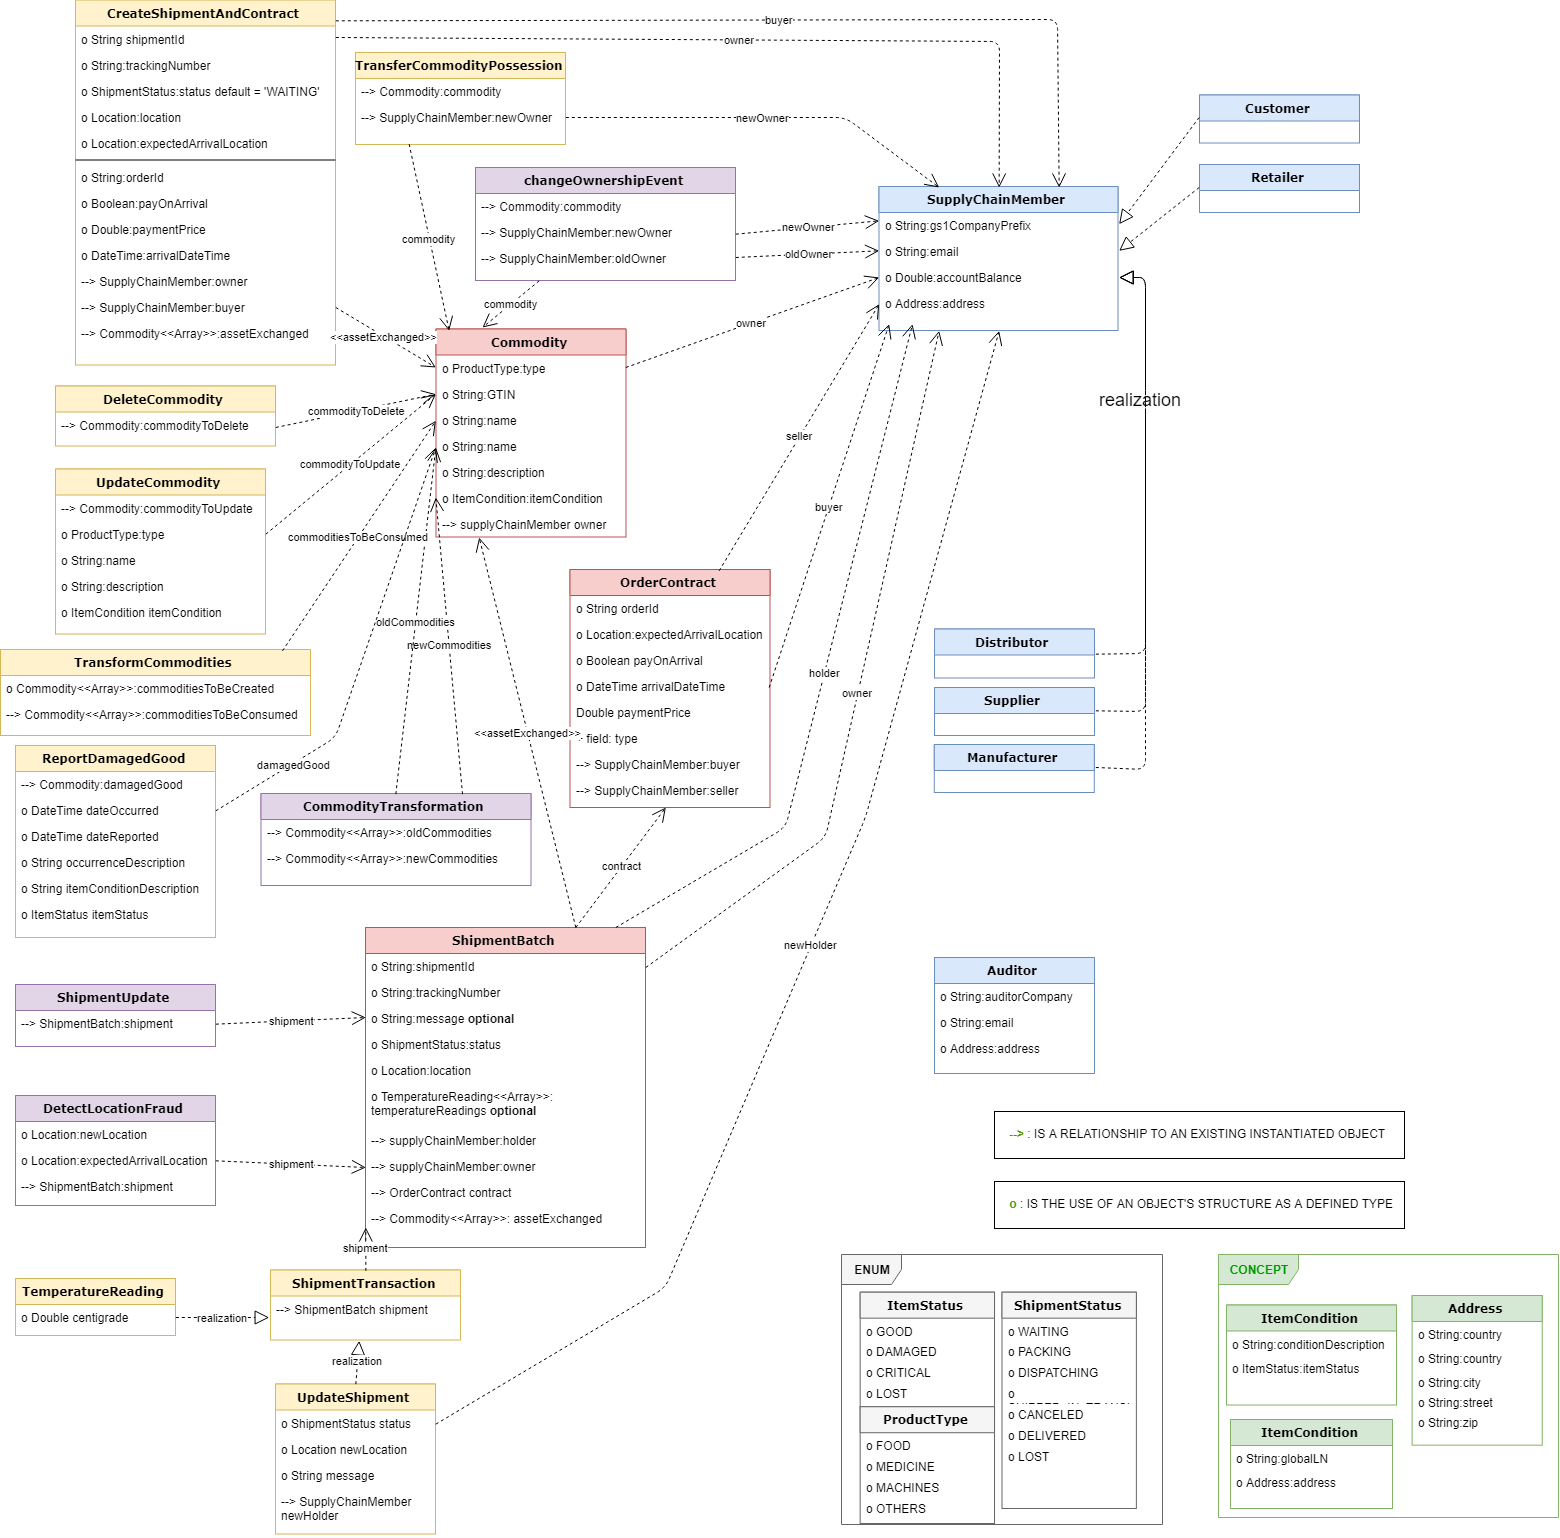
\includegraphics[scale=0.32]{media/full_class_diagram.png}
    \caption[Full class diagram for the designed Hyperledger Composer model]{Full class diagram for the designed Hyperledger Composer model}
    \label{fig:full_class_diagram}
\end{figure}



	% seealso index entries (must come after all other \index calls, so that they appear as the last subitems on index entries)
	%\index{knowledge!capture|seealso{expressiveness}}
	%\index{information|seealso{knowledge, capture}}

	
	\bookmarksetup{startatroot}
	\backmatter
		\cleardoublepage
		\chapter{Publications}
\label{chap:publications}

Many of the materials in this thesis have appeared in the following publications.

\section*{Peer-reviewed Conference Papers}

Lorem ipsum.

\section*{Peer-reviewed Journal Papers}

Lorem ipsum.

\section*{Peer-reviewed Workshop Papers}

Lorem ipsum.

\section*{Peer-reviewed Posters}

Lorem ipsum.

\section*{Doctoral Symposiums}

Lorem ipsum.



		% Glossary
		%\cleardoublepage
		%\phantomsection
		%\begin{singlespace}
		%\begin{footnotesize}
		%\addcontentsline{toc}{chapter}{Nomenclature}
		%\markboth{Nomenclature}{Nomenclature}
		%\makenomenclature
		%% !TEX root = ../thesis.tex

\chapter*{Nomenclature}
\chaptermark{NOMENCLATURE}


\begin{flushleft}
\begin{tabular}{l p{0.8\linewidth}}
	ABB  & Abbreviation
\end{tabular}
\end{flushleft}

		%\printnomenclature[4.5cm]
		%\end{footnotesize}
		%\end{singlespace}

		% Bibliography / References
		\cleardoublepage
		\phantomsection
		\begin{singlespace}
		\begin{footnotesize}
		\addcontentsline{toc}{chapter}{References}
		\bibliographystyle{amsalpha}
		\renewcommand{\bibname}{References}
		\bibliography{references}
		\end{footnotesize}
		\end{singlespace}
		\cleardoublepage
		\phantomsection
		\addcontentsline{toc}{chapter}{Index}
		\printindex
\end{document}
